% Options for packages loaded elsewhere
\PassOptionsToPackage{unicode}{hyperref}
\PassOptionsToPackage{hyphens}{url}
%
\documentclass[
  man]{apa7}
\usepackage{amsmath,amssymb}
\usepackage{iftex}
\ifPDFTeX
  \usepackage[T1]{fontenc}
  \usepackage[utf8]{inputenc}
  \usepackage{textcomp} % provide euro and other symbols
\else % if luatex or xetex
  \usepackage{unicode-math} % this also loads fontspec
  \defaultfontfeatures{Scale=MatchLowercase}
  \defaultfontfeatures[\rmfamily]{Ligatures=TeX,Scale=1}
\fi
\usepackage{lmodern}
\ifPDFTeX\else
  % xetex/luatex font selection
\fi
% Use upquote if available, for straight quotes in verbatim environments
\IfFileExists{upquote.sty}{\usepackage{upquote}}{}
\IfFileExists{microtype.sty}{% use microtype if available
  \usepackage[]{microtype}
  \UseMicrotypeSet[protrusion]{basicmath} % disable protrusion for tt fonts
}{}
\makeatletter
\@ifundefined{KOMAClassName}{% if non-KOMA class
  \IfFileExists{parskip.sty}{%
    \usepackage{parskip}
  }{% else
    \setlength{\parindent}{0pt}
    \setlength{\parskip}{6pt plus 2pt minus 1pt}}
}{% if KOMA class
  \KOMAoptions{parskip=half}}
\makeatother
\usepackage{xcolor}
\usepackage{graphicx}
\makeatletter
\def\maxwidth{\ifdim\Gin@nat@width>\linewidth\linewidth\else\Gin@nat@width\fi}
\def\maxheight{\ifdim\Gin@nat@height>\textheight\textheight\else\Gin@nat@height\fi}
\makeatother
% Scale images if necessary, so that they will not overflow the page
% margins by default, and it is still possible to overwrite the defaults
% using explicit options in \includegraphics[width, height, ...]{}
\setkeys{Gin}{width=\maxwidth,height=\maxheight,keepaspectratio}
% Set default figure placement to htbp
\makeatletter
\def\fps@figure{htbp}
\makeatother
\setlength{\emergencystretch}{3em} % prevent overfull lines
\providecommand{\tightlist}{%
  \setlength{\itemsep}{0pt}\setlength{\parskip}{0pt}}
\setcounter{secnumdepth}{-\maxdimen} % remove section numbering
% Make \paragraph and \subparagraph free-standing
\ifx\paragraph\undefined\else
  \let\oldparagraph\paragraph
  \renewcommand{\paragraph}[1]{\oldparagraph{#1}\mbox{}}
\fi
\ifx\subparagraph\undefined\else
  \let\oldsubparagraph\subparagraph
  \renewcommand{\subparagraph}[1]{\oldsubparagraph{#1}\mbox{}}
\fi
\newlength{\cslhangindent}
\setlength{\cslhangindent}{1.5em}
\newlength{\csllabelwidth}
\setlength{\csllabelwidth}{3em}
\newlength{\cslentryspacingunit} % times entry-spacing
\setlength{\cslentryspacingunit}{\parskip}
\newenvironment{CSLReferences}[2] % #1 hanging-ident, #2 entry spacing
 {% don't indent paragraphs
  \setlength{\parindent}{0pt}
  % turn on hanging indent if param 1 is 1
  \ifodd #1
  \let\oldpar\par
  \def\par{\hangindent=\cslhangindent\oldpar}
  \fi
  % set entry spacing
  \setlength{\parskip}{#2\cslentryspacingunit}
 }%
 {}
\usepackage{calc}
\newcommand{\CSLBlock}[1]{#1\hfill\break}
\newcommand{\CSLLeftMargin}[1]{\parbox[t]{\csllabelwidth}{#1}}
\newcommand{\CSLRightInline}[1]{\parbox[t]{\linewidth - \csllabelwidth}{#1}\break}
\newcommand{\CSLIndent}[1]{\hspace{\cslhangindent}#1}
\ifLuaTeX
\usepackage[bidi=basic]{babel}
\else
\usepackage[bidi=default]{babel}
\fi
\babelprovide[main,import]{english}
% get rid of language-specific shorthands (see #6817):
\let\LanguageShortHands\languageshorthands
\def\languageshorthands#1{}
% Manuscript styling
\usepackage{upgreek}
\captionsetup{font=singlespacing,justification=justified}

% Table formatting
\usepackage{longtable}
\usepackage{lscape}
% \usepackage[counterclockwise]{rotating}   % Landscape page setup for large tables
\usepackage{multirow}		% Table styling
\usepackage{tabularx}		% Control Column width
\usepackage[flushleft]{threeparttable}	% Allows for three part tables with a specified notes section
\usepackage{threeparttablex}            % Lets threeparttable work with longtable

% Create new environments so endfloat can handle them
% \newenvironment{ltable}
%   {\begin{landscape}\centering\begin{threeparttable}}
%   {\end{threeparttable}\end{landscape}}
\newenvironment{lltable}{\begin{landscape}\centering\begin{ThreePartTable}}{\end{ThreePartTable}\end{landscape}}

% Enables adjusting longtable caption width to table width
% Solution found at http://golatex.de/longtable-mit-caption-so-breit-wie-die-tabelle-t15767.html
\makeatletter
\newcommand\LastLTentrywidth{1em}
\newlength\longtablewidth
\setlength{\longtablewidth}{1in}
\newcommand{\getlongtablewidth}{\begingroup \ifcsname LT@\roman{LT@tables}\endcsname \global\longtablewidth=0pt \renewcommand{\LT@entry}[2]{\global\advance\longtablewidth by ##2\relax\gdef\LastLTentrywidth{##2}}\@nameuse{LT@\roman{LT@tables}} \fi \endgroup}

% \setlength{\parindent}{0.5in}
% \setlength{\parskip}{0pt plus 0pt minus 0pt}

% Overwrite redefinition of paragraph and subparagraph by the default LaTeX template
% See https://github.com/crsh/papaja/issues/292
\makeatletter
\renewcommand{\paragraph}{\@startsection{paragraph}{4}{\parindent}%
  {0\baselineskip \@plus 0.2ex \@minus 0.2ex}%
  {-1em}%
  {\normalfont\normalsize\bfseries\itshape\typesectitle}}

\renewcommand{\subparagraph}[1]{\@startsection{subparagraph}{5}{1em}%
  {0\baselineskip \@plus 0.2ex \@minus 0.2ex}%
  {-\z@\relax}%
  {\normalfont\normalsize\itshape\hspace{\parindent}{#1}\textit{\addperi}}{\relax}}
\makeatother

% \usepackage{etoolbox}
\makeatletter
\patchcmd{\HyOrg@maketitle}
  {\section{\normalfont\normalsize\abstractname}}
  {\section*{\normalfont\normalsize\abstractname}}
  {}{\typeout{Failed to patch abstract.}}
\patchcmd{\HyOrg@maketitle}
  {\section{\protect\normalfont{\@title}}}
  {\section*{\protect\normalfont{\@title}}}
  {}{\typeout{Failed to patch title.}}
\makeatother

\usepackage{xpatch}
\makeatletter
\xapptocmd\appendix
  {\xapptocmd\section
    {\addcontentsline{toc}{section}{\appendixname\ifoneappendix\else~\theappendix\fi\\: #1}}
    {}{\InnerPatchFailed}%
  }
{}{\PatchFailed}
\keywords{Gender diversity, Gender categorization, Transgender, Measurement\newline\indent Word count: 3969}
\DeclareDelayedFloatFlavor{ThreePartTable}{table}
\DeclareDelayedFloatFlavor{lltable}{table}
\DeclareDelayedFloatFlavor*{longtable}{table}
\makeatletter
\renewcommand{\efloat@iwrite}[1]{\immediate\expandafter\protected@write\csname efloat@post#1\endcsname{}}
\makeatother
\usepackage{csquotes}
\makeatletter
\renewcommand{\paragraph}{\@startsection{paragraph}{4}{\parindent}%
  {0\baselineskip \@plus 0.2ex \@minus 0.2ex}%
  {-1em}%
  {\normalfont\normalsize\bfseries\typesectitle}}

\renewcommand{\subparagraph}[1]{\@startsection{subparagraph}{5}{1em}%
  {0\baselineskip \@plus 0.2ex \@minus 0.2ex}%
  {-\z@\relax}%
  {\normalfont\normalsize\bfseries\itshape\hspace{\parindent}{#1}\textit{\addperi}}{\relax}}
\makeatother

\ifLuaTeX
  \usepackage{selnolig}  % disable illegal ligatures
\fi
\IfFileExists{bookmark.sty}{\usepackage{bookmark}}{\usepackage{hyperref}}
\IfFileExists{xurl.sty}{\usepackage{xurl}}{} % add URL line breaks if available
\urlstyle{same}
\hypersetup{
  pdftitle={Inclusive Response Options Expand Gender Categorization But Do Not Reduce Categorical Perception of Gender},
  pdfauthor={Elli van Berlekom1, Stefan Wiens1, Anna Lindqvist2, \& Marie Gustavsson Sendén1},
  pdflang={en-EN},
  pdfkeywords={Gender diversity, Gender categorization, Transgender, Measurement},
  hidelinks,
  pdfcreator={LaTeX via pandoc}}

\title{Inclusive Response Options Expand Gender Categorization But Do Not Reduce Categorical Perception of Gender}
\author{Elli van Berlekom\textsuperscript{1}, Stefan Wiens\textsuperscript{1}, Anna Lindqvist\textsuperscript{2}, \& Marie Gustavsson Sendén\textsuperscript{1}}
\date{}


\shorttitle{Rsponse options and gender categorization}

\authornote{

Data \& scripts are available at figshare. The authors declare no conflict of interest.

The authors made the following contributions. Elli van Berlekom: Conceptualization, Data collection, Data analysis, Writing - Original Draft Preparation, Writing - Review \& Editing; Stefan Wiens: Data analysis, Writing - Review \& Editing; Anna Lindqvist: Conceptualization, Writing - Review \& Editing; Marie Gustavsson Sendén: Conceptualization, Writing - Review \& Editing.

Correspondence concerning this article should be addressed to Elli van Berlekom, Albanovägen 12. E-mail: \href{mailto:elli.vanberlekom@psychology.su.se}{\nolinkurl{elli.vanberlekom@psychology.su.se}}

}

\affiliation{\vspace{0.5cm}\textsuperscript{1} Stockholm University\\\textsuperscript{2} Lund University}

\begin{document}
\maketitle

The experiences of transgender and gender diverse (TGD) individuals suggest that many people experience gender as fluid, diffuse, and not bounded by the typical western binary of women and men Hyde et al. (2018). In surveys and questionnaires, however, gender is often constructed as a binary by limiting ther esponse options to the categories to woman/female and man/male (Saperstein \& Westbrook, 2021). Such measurement invisibilise and and implicitly deligitimze TGD identities (Ansara \& Hegarty, 2014). Recently, calls have gone out urging psychologists to include a wider range response options (e.g, nonbinary, other, ref) or using free text options (Lindqvist et al., 2020) practices which are becoming widely adopted (ref). {[}gender is still binary, other perception{]}. Research on gender categorization of others, however, is is still dominating by binary thinking (for example). Here we report two studies demonstrating how gender categorization of faces can be measured without reinforcing binary gender norms and such measurements do and do not affect participants' responses.

\hypertarget{measuring-self-identified-gender}{%
\subsection{Measuring self-identified gender}\label{measuring-self-identified-gender}}

An early example of a radical measurement of gender binary was Sandra Bem who argued that femininity and masculinity are not mutually exclusive and need to be measure separately (bem). Using Bem's scale, the Bem Sex-Role Inventory (BSRI), a person could score highly on both femininity and masculinity, or low on both, implying a level of flexibility in gender traits. This challenged the prevailing norm of thinking about gender as a strict and mutually exclusive binary. This bidimensional approach has been cited as significant milestone in progressive measurement (queering bem).

Characteristically for western research of it's time, however, Bem's work was still largely carried out within a binary gender framework, even as it implicitly challenged that framework. The BSRI defined gender as a psychological trait and the people possessing those traits were still seen as exclusively women or men. Since then, as the extent of gender diversity has become more widely known (national geographic), it has become widely understood that any measurement which does not take this gender diversity into account is insufficient on its own. That said, this has not stopped many people from citing Bem's bidimensional conception as a model for other types of gender research.

Later recommendations have suggested ways to measure gender as a discrete category while still enabling participants to choose from a diversity of identities. For example, Saperstein and Westbrook (2021) suggested that surveys measuring gender include a range of response options, such as non-binary, other, transman, agender and more. Taking a slightly different approach, Lindqvist et al.~(2020) suggested an open text entry where participants can fill in whatever. This, they argue, has the most benefits to respondents. The free text response has the advantage of being completely unconstrained, allowing participants to enter any category, including categories which may not have occurred to the researchers. Moreover, the acceptable terms sometimes shift over time, as more marginalized voices are heard. The term ``transsexual'' for example, was widely used and seen as acceptable, but is now understood to be stigmatizing (APA manual). A free text easily sidesteps this issue. It is increasingly common among researchers to adopt these open-ended approaches to measure participant gender (e.g. Carleton et al., 2022; Cronin et al., 2022; D'Agostino et al., 2022; Göttgens et al., 2022).

Until now, most recommendations primarily suggest ways to measures participants' own gender. This emphasis is understandable as gender identity is a commonly reported demographic variable. But gender is frequently is also frequently measured in terms of participants categorizations of others. The form such measurement takes is often quite similar to self-categorization, usually a forced-choice selection of a number of named categories. Because self-categorization and categoriztion of others are different processes, however, it is not immediately clear that the best way to measure self-categorization also applies to categorization of others.

\hypertarget{measuring-gender-categoriztion-of-others}{%
\subsection{Measuring gender categoriztion of others}\label{measuring-gender-categoriztion-of-others}}

One important consideration for face perception is the morphology of faces. Faces are frequently described as dimorphic, in other words that they typically manifest in two distinct types of forms. The faces of men and women differ on average (Zaidi, Mitteroeker). Specific features of faces, such as jawline, eyebrow shape and hairline tend to be associated with either women or men (Brown \& Perrett). That said a big part of what is considered gender in faces can be boiled down to just differences in size (Mitteroecker). Additionally, there is substantial variation in gendered features even within the binary gender categories. When these features are analyzed independently, the differences in gender are less pronounced, challenging the notion of strict facial dimorphism.

Despite this, research on how people perceive and categorize the gender of others still almost exclusively treats gender as a binary category. The most common way to do this is by showing people a face and asking them to categorize the faces as either a man or a woman. Using this method, research has shown that people rapidly and automatically categorize gender (Habibi \& Khurana, 2012; Jung et al., 2019), according facial features such as skin smoothness, jawline, and hair length used to determine gender identity. Morever, particpants categorize faces categorically (Campanella et al., 2001). This phenomenon has been observed when participants categorize a number of faces that have been morphed to vary unidimensionally from feminine to masculine. Categorizations of these morphed faces were accentuated towards the dominant gender of the face, so that for example a 60\% female morph was rated as a woman by closer to 80\% of participants (Campanella et al., 2001).

However, measuring gender categorization as a binary category or on a unidimensional scale does not accurately reflect the diversity of gender as it is experienced by many people (Hyde et al., 2018). By creating a binary out of a more varying dimension, researchers and data collector miss variation, similar to how measurement of age as only ``young'' or ``old'' would miss the variation of ages.

Moreover, the inclusion or exclusion of certain response options communicates certain ideas to participants. Binary response options suggests that women and men are the only two genders just as multiple options imply that gender is more diverse. In other words, no matter which type of response options are used, some ideas are being communicated to participants, potentially introducing a bias in their responses. Researchers are typically wary of biasing participants (ref), but the effects of gender response options are rarely considered. Binary and unidimensional response options, for example, may bias participants toward conceiving of gender as a binary category. Non-binary, or bidimensional response options, on the other hand, could have an opposite effect. Additionally, if for example masculine faces, are more likely to be categorized as non-binary, this would in practice bias overall categorizations toward women.

Furthermore, given the increasing diversity in gender identity, understanding the for categorizing of individuals as beyond the traditional binary framework is emerging as a an area of research unto itself. However, being a relatively unexplored domain, effective methodologies for measuring these categorizations are not well-established. This study aims to address this significant gap by identifying more accurate and comprehensive methods for gender categorization analysis.

\hypertarget{the-present-research}{%
\subsection{The present research}\label{the-present-research}}

The aim of this study is to broadly how various inclusive and non-binary response options affect the perception and categorization of gender of faces. In Study 1 we measured perceptions of gender as a unidimensional and bidimensional construct. We investigated whether the rated gender was accentuated compared to physical of the faces gender indicating categorical perception (Research Question 1) and whether this categorical perception was heightened when gender was measured as unidimensional construct compared to when it was measured as a bidimensional construct (Research Question 2). In Study 2 we measured perceptions of gender measured as discrete categories. We investigated whether and how often participants categorized faces beyond the binary when categorizing faces using inclusive response options (Research Question 3). Additionally, we investigated how inclusive options influenced categorization of faces as women and men (Research Question 4).

\hypertarget{study-1}{%
\section{Study 1}\label{study-1}}

Study 1 tested how gender is perceived when response options are either unidimensional or bidimensional The basis for the study is the pioneering work of Bem (1974) that highlighted the importance of measuring gender as a continuum rather than as discrete categories, and that femininity and masculinity might not be end points on the same continuum. Although Bem was primarily interested in the measurement of participant own gender, more recent recommendations have suggested continuous measurement as suitable method for any measure of gender, including perceptions of gender of others (Hyde et al., 2018). Study 1 explored the use of continuous measurement of gender in terms of two outcomes: a single woman-man continuum and separate man/women continua.

Using morphed faces, we examined the phenomenon of categorical gender perception, wherein participants tend to perceive more gender in a face than is actually present. The consequence of this effect is that that participants, when presented with faces displaying subtle gender cues, still categorize them as distinctly female or male. For example, a face with 66\% facial femininity should be perceived as female, while a face with 33\% facial femininity should be perceived as male. Study 1 examined whether this effect would be observed using a continuous gender rating (Research Question 1). Furthermore, we explored whether employing response options that do not frame women and men as opposites would diminish the accentuated gender perception (Research Question 2).

\hypertarget{method}{%
\section{Method}\label{method}}

\hypertarget{participants}{%
\subsubsection{Participants}\label{participants}}

Swedish participants (\emph{N} = 66) were recruited through advertising online and on the university campus (\emph{M}\textsubscript{age}= 37.36, \emph{SD}\textsubscript{age} = 14.14, Range = 18 - 73). Self-identified gender was measured using an open-ended text box (31 women, 32 men and 2 participants who did indicate gender). Participants were monetarily compensated for their time (100 sek). All participants were informed that participation was voluntary and gave written consent to participate in the study in accordance with ethical recommendations. The participants were randomly allocated to conditions.

\hypertarget{stimuli}{%
\subsection{Stimuli}\label{stimuli}}

The experiment included faces from the London Face Database (L. M. DeBruine \& Jones, 2017) and the Chicago Face Database (Ma et al., 2015) morphed with on Webmorph (L. DeBruine, 2018). For Black, Asian and White faces, the six most feminine faces of women and the six most masculine faces of men were selected, using the codebook provided by the researchers. The faces were matched, so that the most feminine faces in the database were morphed with the most masculine faces. The morphs were made in 7 steps, from completely feminine to completely masculine. We defined the morph level as the degree of the the female face present in the morph. In other words, a 33.33\% was slightly tilted toward the man, a 50\% face was an even mixture and a 100\% consisted only of the woman's face. Because there were 18 pairs morphed in 7 steps, the total number of faces was 126.

\begin{figure}
\hypertarget{fig-stimuli}{%
\centering
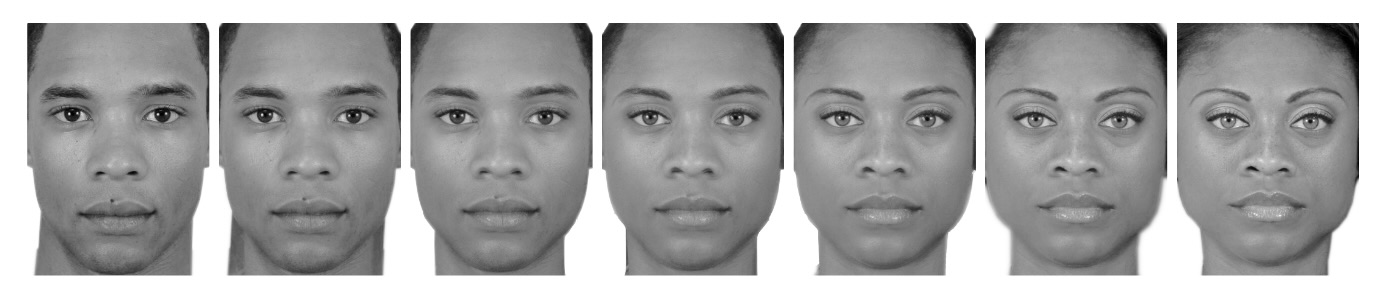
\includegraphics{pix/stimuli.jpeg}
\caption{Example of seven step morphing spectrum}\label{fig-stimuli}
}
\end{figure}

\hypertarget{design-and-procedure}{%
\subsection{Design and procedure}\label{design-and-procedure}}

The experiment used a between-participants design with two response options conditions. These were the \emph{unidemnsional}, and \emph{bidimensional} and conditions. Participants were randomly allocated into one of the two response options conditions.

Participants completed the experiment on a computer in a quiet room. Each trial consisted of a face accompanied by the question ``How would you gender categorize this person?''. In the single dimension condition, participants rated gender based on a single continuum with the anchors marked ``woman'' and ``man''. In the multiple dimensions condition, participants rated each face twice on two different continua, ranging from ``not woman'' or ``not man'' to ``woman'' or ``man''. Each person completed a total of 126 trials (i.e.~they categorized every face in the stimuli set).

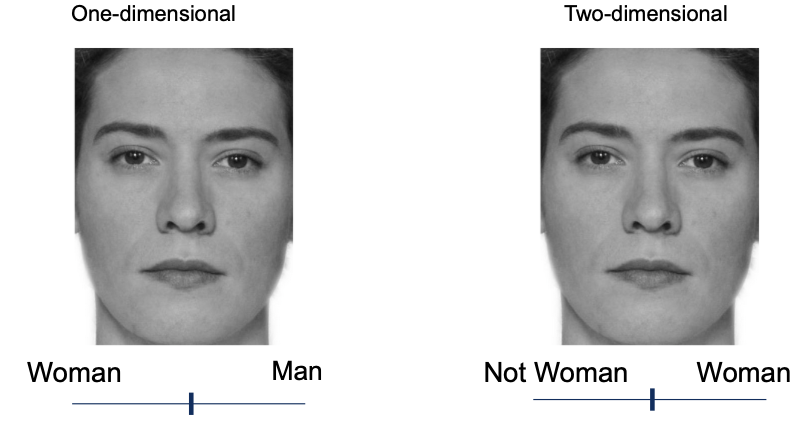
\includegraphics{pix/exp2.png}{]}

\hypertarget{data-analysis}{%
\subsection{Data analysis}\label{data-analysis}}

Descriptive statistics highlight individual participants tendency toward categorical perception. Bayesian mixed-effects models were used to test categorical perception between conditions (Research Question 2). In all models, morph level and condition were included as fixed effects. Additionally, all models included varying intercepts for both participants and trials and varying slopes for facial femininity. The pattern of scores were clearly non-linear, meaning any linear model would probably be misspecified. Therefore, to reduce the complexity of the model, facial femininity was modeled as an ordered factor with seven levels, corresponding to each of the seven morphing steps. Any categorical perception effects should be strongest closest to the midpoint, therefore, we compared the two conditions at morph level = 33.37 and 66.66, reporting the credible intervals of the difference as well as the Savage-Dickey Bayes factors.

\hypertarget{results}{%
\section{Results}\label{results}}

\hypertarget{was-gender-percieved-categorically-research-question-1}{%
\subsection{Was gender percieved categorically? (Research Question 1)}\label{was-gender-percieved-categorically-research-question-1}}

To investigate whether participants categorized gender categorically to the morph level (i.e.~degree of gender. ) of the faces we visualized responses in Figure\ref{fig:descriptives-two}. If participants respond only to the morph of faces, the lines should be a straight diagonal. Instead, Figure\ref{fig:descriptives-two} shows that most participants display a non-linear S-shape (see the light lines) and this was indeed also the pattern of the group means in both conditions (see the dark lines). However, the Figure\ref{fig:descriptives-two} also suggests that there was a high degree of individual variation, and some participants were more categorical than others in their ratings.

\begin{figure}
\centering
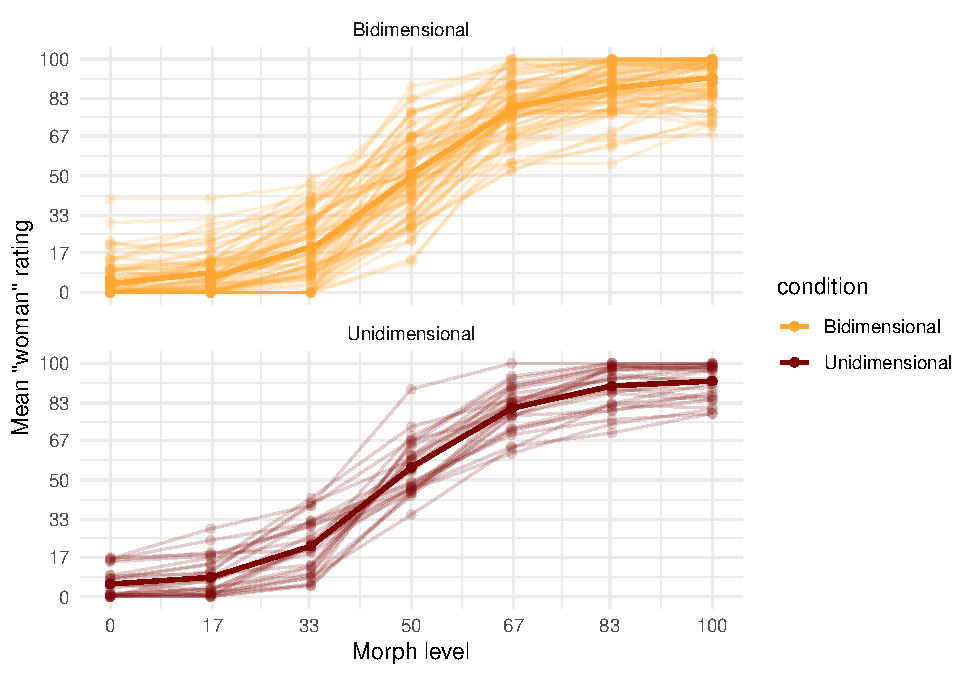
\includegraphics{RO_revisions_doc_files/figure-latex/descriptives-two-1.pdf}
\caption{\label{fig:descriptives-two}Participant level and mean ratings of faces in Single dimension and multiple dimensions}
\end{figure}

\hypertarget{is-there-a-difference-in-accentuated-perception-by-condition-research-question-2}{%
\subsection{Is there a difference in accentuated perception by condition? (Research Question 2)}\label{is-there-a-difference-in-accentuated-perception-by-condition-research-question-2}}

We tested whether this accentuation effect was stronger in the unidimension condition compared to the bidimensional condition. If bidimensional response options reduced categorical perceptions, ratings of femininity roughly equal to the morph level 33 and lower at morph level 66, or at least more equal than in the unidimensional condition. To test this, we modelled the data as bayesian mixed effects models, with each level of facial femininity as a factor.

\begin{figure}
\centering
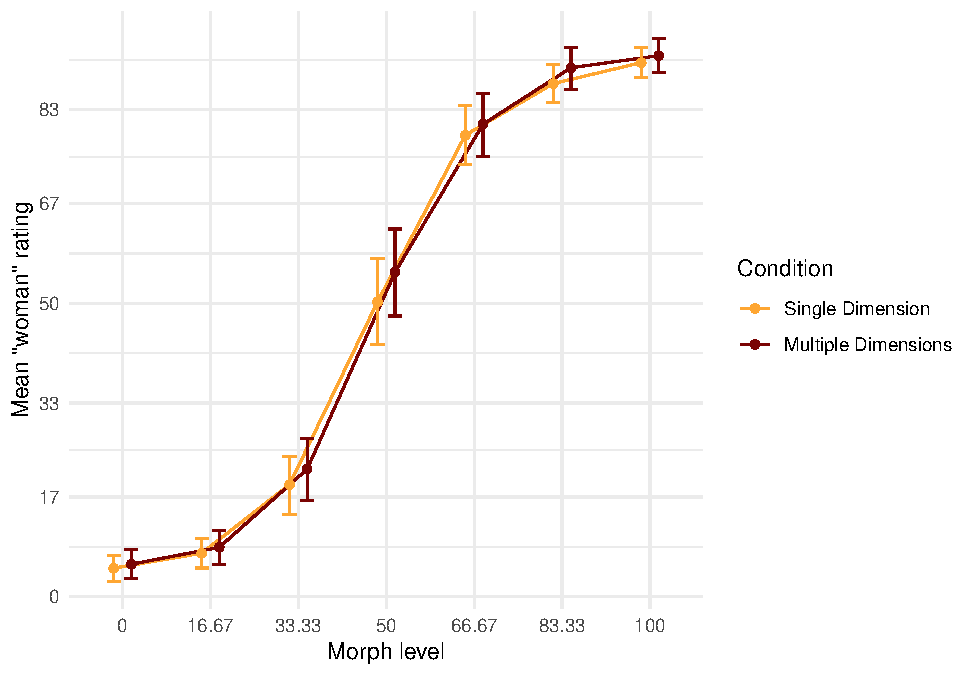
\includegraphics{RO_revisions_doc_files/figure-latex/exp-two-inf-1.pdf}
\caption{\label{fig:exp-two-inf}Mean gender ratings in Single Dimension and Multiple Dimensions conditions}
\end{figure}

We compared the mean rating at morph levels 33.33 and 66.67 morph for both conditions. At morph level 33.33 the evidence strongly suggested that the mean ``woman rating'' in was the same in the Unidemensional () and Bidimensional conditions () (Estimate = -2.63, CI =\[-7.93, 2.76\], BF\textsubscript{01}= 17.10). This was also the case at morph level 66.67 (Estimate = -1.79, CI =\[-6.31, 2.77\], BF\textsubscript{01}= 23.55). Overall, both conditions showed fairly strong tendencies toward accentuated gender perception and they did not differ in this regard. In other words, for face perception we did not find that a bidimensional rating scale reduced categorical perception.

\hypertarget{discussion}{%
\subsection{Discussion}\label{discussion}}

Study 2 showed that participants exhibited signs of categorical gender perception when rating faces in terms of gender. Additionally, this did not depend on response option condition; response options which did not present women and men as opposing categories led to an equal amount of accentuated perception as response options that did. Indeed a highly binary view of gender was present and participants treated womanhood and manhood as opposites even the scale would allow them to be more flexible.

\hypertarget{study-2}{%
\section{Study 2}\label{study-2}}

Study 2 adapted common ways to measure participants categorization of their own gender to other categorization research. One common recommendation is to include a third option gender option, such as ``non-binary'' or ``other''. Another common practice is to give people an open text box in which they may type in whatever they like (Lindqvist et al., 2020; Saperstein \& Westbrook, 2021). Therefore, Study 2 compared the standard binary response options to two alternatives: a third gender option (such as `non-binary' or `other') and an open text box for participants to type in their gender. An important difference between self-categorization and the categorization of others is that most people know their own gender, whereas the gender of others cannot always be known from appearance (Richards et al., 2016). To account for this, we also gave participants the ability to state that gender was unknown.

\hypertarget{method-1}{%
\section{Method}\label{method-1}}

\hypertarget{participants-1}{%
\subsection{Participants}\label{participants-1}}

Swedish participants (\emph{N} = 100) completed the study in a lab at a Stockholm University campus (\emph{M}\textsubscript{age}= 37.16, \emph{SD}\textsubscript{age} = 13.89, Range = 18 - 69). Self-identified gender was measured using an open-ended text box as recommended by Lindqvist et al. (2020) (56 women, 47 men 2 who did not indicate). All participants were informed that participation was voluntary, that they could withdraw from the study and that results do no include any identifying features. All participants provided written informed consent.

\hypertarget{design-stimuli-and-procedure}{%
\subsection{Design, Stimuli and Procedure}\label{design-stimuli-and-procedure}}

The experiment used a between-participants design with three response options conditions. These were the \emph{binary categories}, \emph{free text} and \emph{multiple categories} and conditions. The administering researcher was blind to participant condition and participants were randomly allocated into one of the three experimental conditions. Participants were randomly allocated into one of the three response options conditions: binary categories, multiple categories, and free text (see (\textbf{fig-exp1-trial?})). In the binary categories condition the response options consisted of two categories: ``woman'' and ``man''. In the free text condition the response options consisted of an open text box. In the multiple categories condition, the response options consisted of four categories: ``woman'', ``man'', ``other'' and ``I don't know''. The stimuli were identical to those of Study 1. After being allocated to one of the three conditions, participants categorized 126 faces according to the response options in their condition.

\begin{figure}
\hypertarget{fig-exp1-trial}{%
\centering
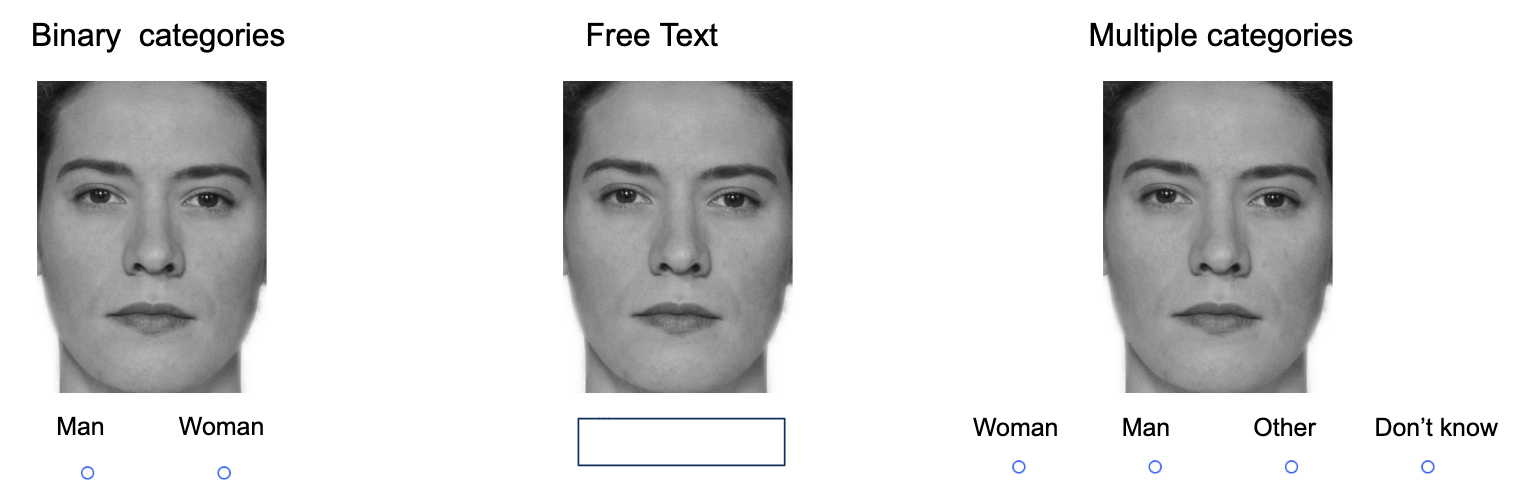
\includegraphics{pix/exp1.png}
\caption{Sample trial from each of the three conditions}\label{fig-exp1-trial}
}
\end{figure}

\hypertarget{measures}{%
\subsection{Measures}\label{measures}}

The primary outcome was responses to the categorization task. For analysis purposes, these were aggregated in the following ways:

\emph{Beyond-binary categorizations} represented the categories where participants did not categorize the face as woman or man. This was a dichotomous variable that was calculated from the categorization data by combining the responses of ``I don't know'' and ``other'' in the multiple categories condition. In the free text condition, this included various variations of ``other'' and ``non-binary''. These beyond-binary responses were coded as 1 and binary responses as 0.

\emph{Binary categorization} represented only the responses that were either woman (coded as 1) or man (coded as 0). All other responses were removed from this dataset.

\hypertarget{data-analysis-1}{%
\subsection{Data analysis}\label{data-analysis-1}}

We used R (Version 4.2.2; R Core Team, 2022) and the R-packages \emph{brms} (Version 2.18.0; Bürkner, 2017, 2018, 2021), \emph{papaja} (Version 0.1.1; Aust \& Barth, 2022), and \emph{tidyverse} (Version 1.3.2; Wickham et al., 2019). Additionally, much of the R code was adapted from Kurz (2023) . Descriptive statistics were used to summarize the data, and Bayesian mixed-effects models were used to test research questions 2. In all models, facial femininity and condition were included as fixed effects. Additionally, all models included varying intercepts for both participants and trials and varying slopes for facial femininity. To answer each research question, we used a two-step approach which began with a model comparison approach followed by Bayes factor tests of specific contrasts.

\hypertarget{results-1}{%
\section{Results}\label{results-1}}

\hypertarget{how-does-inclusive-response-options-affect-categorizations-beyond-the-binary-research-question-3}{%
\subsection{How does inclusive response options affect categorizations beyond the binary (Research Question 3)}\label{how-does-inclusive-response-options-affect-categorizations-beyond-the-binary-research-question-3}}

The raw distribution of gender categorizations made by participants is presented in Figure~\ref{fig:descriptives}.

\begin{figure}
\centering
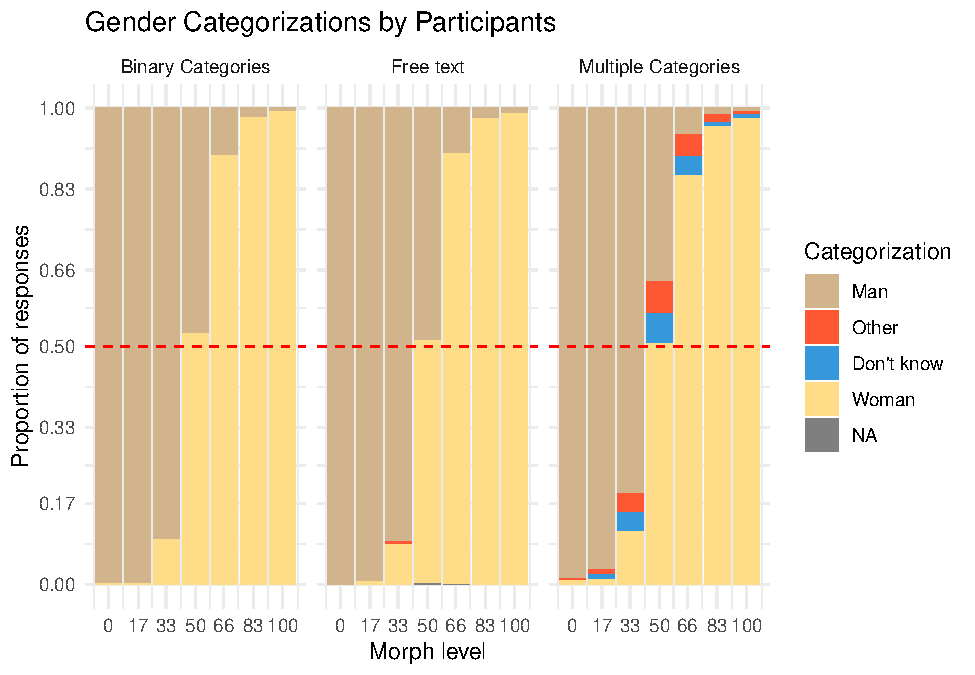
\includegraphics{RO_revisions_doc_files/figure-latex/descriptives-1-1.pdf}
\caption{\label{fig:descriptives-1}Gender Categorizations by Participants}
\end{figure}

We investigated whether participants categorized faces beyond the binary when given the option to do so (Research Question 3). To do this, we plotted the distribution of categorizations for each participant (see Figure\ref{fig:descriptives}.)

Even when participants had the option to categorize face beyond the binary, most still categorized faces as women and men. In the free text condition, only one participant categorized a single face as other than woman and man. In the multiple categories condition, around half of participants categorized any face beyond the binary see figure XX. Even among participants who categorized any faces beyond the binary, there was a great deal of variation in tendency to use these categories (see figure 3)

\emph{here are two version of the same figure. I don't quite understand why the numbers don't add up though. I'll have to do some more digging in the code. }

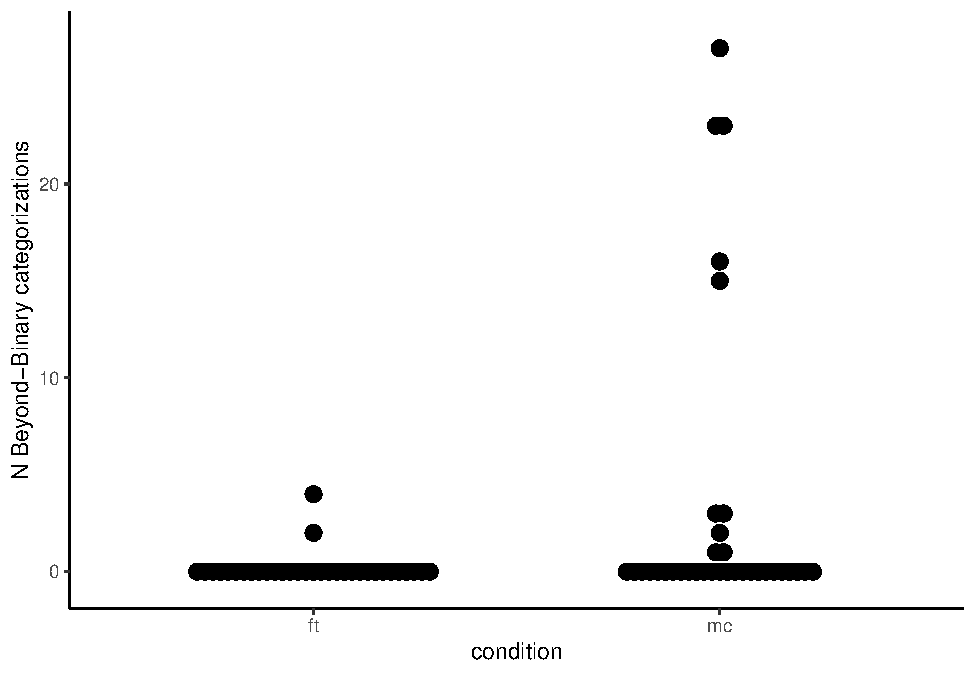
\includegraphics{RO_revisions_doc_files/figure-latex/unnamed-chunk-5-1.pdf} 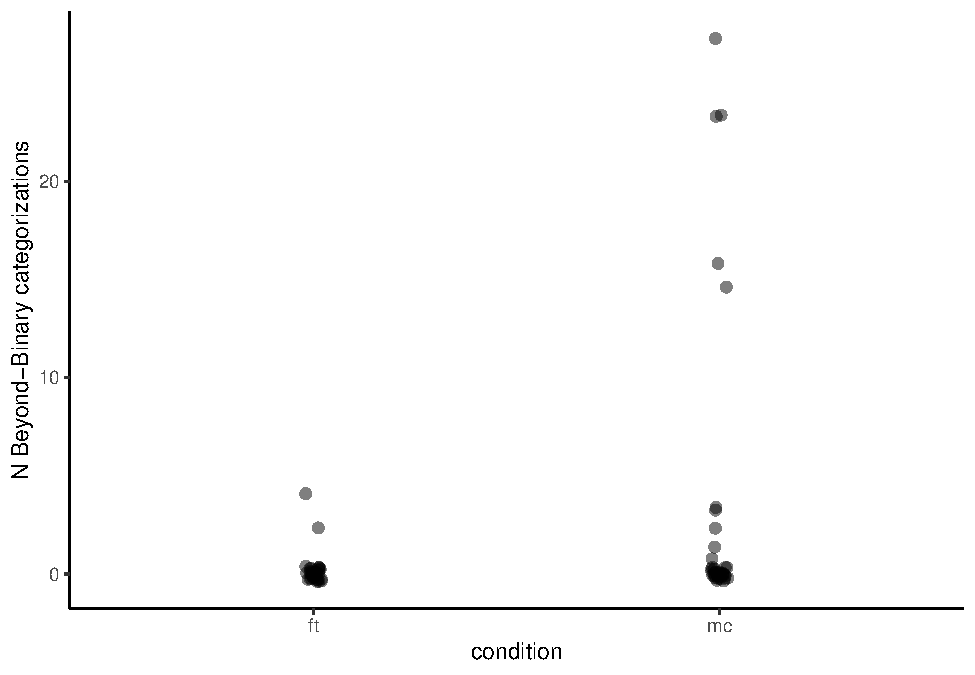
\includegraphics{RO_revisions_doc_files/figure-latex/unnamed-chunk-5-2.pdf}

\hypertarget{categorization-of-women-and-men-research-question-4}{%
\subsection{Categorization of women and men (Research Question 4)}\label{categorization-of-women-and-men-research-question-4}}

When people categorize faces beyond the binary such categorization also affects the categorization of faces as men or women. For example, does categorization of faces as non-binary systematically replace ``woman'' categorization. As non-binary options have been promoted by feminist and LGBTQ+ activists, their inclusion might have more generalized effects on binary categorization. We therefore investigated inclusive response options changed participants overall tendency to categorize women and men. Descriptive statistics for individual level responses are displayed in figure X

\begin{figure}
\centering
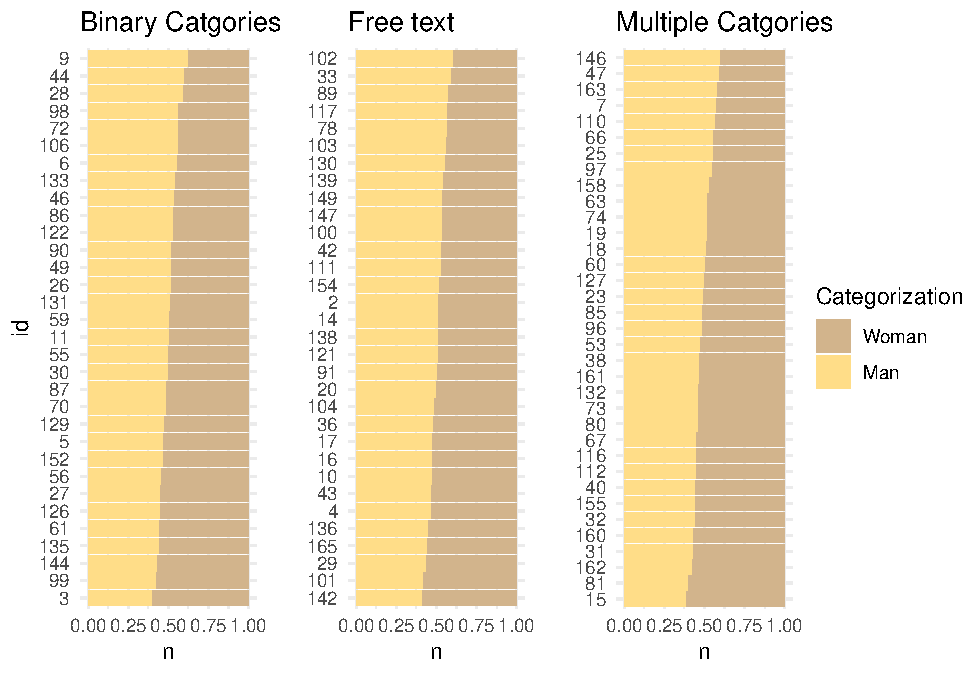
\includegraphics{RO_revisions_doc_files/figure-latex/descriptivesx-1.pdf}
\caption{\label{fig:descriptivesx}Binary Gender Categorizations by Participants in the three conditions (non-binary responses were excluded)}
\end{figure}

This was tested by fitting a Bayesian mixed effects model to the data. In addition to random intercepts for participants and random slopes for facial femininity, the model included a fixed effect of condition, and unique slopes of facial femininity for each condition (see supplementary material).

The comparison of the multiple categories condition and the binary categories condition, indicated moderate evidence that gender categorization in the two conditions were the same (OR = 0.68, CI =\[0.40, 1.17\], BF\textsubscript{01}= 5.94). The comparison of the free text and binary categories conditions indicated strong evidence that the two conditions were the same (OR = 1.03, CI =\[0.60, 1.78\], BF\textsubscript{01}= 15.42). In other words, neither the free text or the multiple categories condition changed the pattern of categorization of women and men compared to the binary categories condition.

We also compared the relationship between facial femininity and woman categorizations (i.e.~the slope of facial femininity) across the conditions. The effect of facial femininity on woman categorizations was almost exactly the same in the multiple categories and binary categories, as there was overwhelming evidence in favor of no difference (Difference = 0, CI =\[-0.02, 0.03\], BF\textsubscript{01}= 398.85). The effect of facial femininity on woman categorizations almost was exactly the same in the free text and binary categories, as there was overwhelming evidence in favor of no difference ((Difference = 0, CI =\[-0.02, 0.02\], BF\textsubscript{01}= 398.85) )

\hypertarget{discussion-1}{%
\section{Discussion}\label{discussion-1}}

Experiment 1 indicated that participants categorize beyond the binary when response options include more options than women and men only. However, the free text option did not differ from the binary option. Thus, the written out choices seem to act as reminders to participants. Furthermore, categorization beyond the binary affected former man and women responses to similar degrees, meaning that the ratio of women and men categorizations was still about 50/50. This did not systematically affect their overall pattern of responses in terms of woman and man categorizations.

\hypertarget{general-discussion}{%
\section{General discussion}\label{general-discussion}}

This study aimed to test how different response options of gender categorization influence how gender is perceived. In study 1 we compared uni-dimensional and two-dimensional continuous scales, and in Study 2, we compared binary (traditional) response options, with multiple categories and free-text answers. In both studies we used a multiracial set of morphed faces to show responses to a variety of femininity and masculinity in faces.

We found a strong tendency for binary perceptions of gender, both in terms that people accentuate their perceptions of womanhood and manhood when rating gender on continuous scales (Study 1), and that people that have the possibility to indicate other gender than woman or man seldomly do so (Study 2). However, we also found that multiple opitions made people aware of byeound binary gender to a rather high degree in that 50 \% \ldots. Fre text options did not hae such an effect.

In two experiments, we tested how response options in gender categorization of others influence gender categorization and accentuated perception of gender. The results suggested that about half of participants categorized gender beyond the binary when presented with non-binary alternatives, but that almost none do it when using a free text response. The results also suggested the presence of non-binary categorizations replaced categorizations of women and men equally. Furthermore, when participants rated gender on a continuum, there was still a tendency toward categorical perception of gender, though not for every participant. Lastly, participants exhibited similar levels of categorical perception in both the unidimensional and bidmensional conditions.

The finding that participants use non-binary response options are somewhat consistent with previous research, such as the work of Saperstein and Westbrook (2021) and Lindqvist et al. (2020), which has shown that including flexible response options allow participants to better express themselves. Unlike the literature on self-categorization, increased freedom did not increase the gender diversity of participants' categorizations. This likely reflects the difference between categorizing oneself and categorizing others. Non-binary are likely to be hyper-aware of their own non-binary gender identity (Richards et al,) whereas cisgender participants are seemingly not as likely to think about. It may also be the case that particiants are not aware that categorizing beyond the binary was not an option.

When participants categorized women or men on continuous scales, the results differ from Bem (1974) who found that participants categorize their own femininity and masculinity independently of each other. Rather, when categorizing others, the participants in the present study seemed to treat women and men as opposites, even when the response options did not pose them as such. Both of these deviations from the previous literature likely stem from the substantial difference between indicating one's own gender and categorizing that of others.

It is worth noting that this study only examined participants' stated categorizations, and it is possible that they may have made other categorizations internally that were not reflected in their responses. However, it is important to recognize that a purely behavioral study such as this cannot fully capture the neurological processes underlying gender perception, which may require more sophisticated techniques such as EEG and eye-tracking (Kloth et al., 2010; Stolier \& Freeman, 2017).

In this study we aggregated responses that did not indicate woman or man. In the multiple response option condition, both ``I don't know'' and ``Non-binary'' were included as a beyond binary categorization. We justified this on the basis that what we were interested in is any categorization beyond the binary. However, these two options are not the same. Furthermore, it is important to note that many non-binary individuals do not have a prototypically androgynous gender expression (Richards et al., 2016). Therefore, if a person aims to be inclusive and not categorize in a binary way, then abstaining from categorizing, for example by selecting ``I don't know'' is always the best option.

In the introduction we raised the possibility that findings within gender categorization research may be biased from a sole reliance on binary response options. Based on the present results, this seems unlikely. Instead, it seems that the societal norm to treat gender as binary is the strongest determinant participants gender categorizations. Even so, we recommend researchers to carefully consider their measurements of gender categorization. Open text-boxes, forced choice-alternatives and continua are all viable alternatives. Even researchers who are primarily interested in binary categorizations should consider including beyond-binary alternatives, to avoid perpetuating the binary gender norm and to accurately represent the diversity of gender.

\hypertarget{conclusion}{%
\paragraph{Conclusion}\label{conclusion}}

In two experiments we tested how different response alternatives affected gender categorizations. Participants were more likely to categorize faces beyond the binary when using a forced-choice paradigm including ``non-binary'' and ``I don't know'' than when using a free text option, or slider scales. In comparison to self-identification questions where open ended responses are seen as the most inclusive alternative (Lindqvist et al., 2020), categorization of others benefit from response options that explicitly reminds participants that not all people identify as women or men.

\newpage

\hypertarget{references}{%
\section{References}\label{references}}

\hypertarget{refs}{}
\begin{CSLReferences}{1}{0}
\leavevmode\vadjust pre{\hypertarget{ref-ansara_methodologies_2014}{}}%
Ansara, Y. G., \& Hegarty, P. (2014). Methodologies of misgendering: Recommendations for reducing cisgenderism in psychological research. \emph{Feminism \& Psychology}, \emph{24}(2), 259--270. \url{https://doi.org/10.1177/0959353514526217}

\leavevmode\vadjust pre{\hypertarget{ref-R-papaja}{}}%
Aust, F., \& Barth, M. (2022). \emph{{papaja}: {Prepare} reproducible {APA} journal articles with {R Markdown}}. \url{https://github.com/crsh/papaja}

\leavevmode\vadjust pre{\hypertarget{ref-bem_measurement_1974}{}}%
Bem, S. L. (1974). \emph{{THE} {MEASUREMENT} {OF} {PSYCHOLOGICAL} {ANDROGYNY}}. 8.

\leavevmode\vadjust pre{\hypertarget{ref-R-brms_a}{}}%
Bürkner, P.-C. (2017). {brms}: An {R} package for {Bayesian} multilevel models using {Stan}. \emph{Journal of Statistical Software}, \emph{80}(1), 1--28. \url{https://doi.org/10.18637/jss.v080.i01}

\leavevmode\vadjust pre{\hypertarget{ref-R-brms_b}{}}%
Bürkner, P.-C. (2018). Advanced {Bayesian} multilevel modeling with the {R} package {brms}. \emph{The R Journal}, \emph{10}(1), 395--411. \url{https://doi.org/10.32614/RJ-2018-017}

\leavevmode\vadjust pre{\hypertarget{ref-R-brms_c}{}}%
Bürkner, P.-C. (2021). Bayesian item response modeling in {R} with {brms} and {Stan}. \emph{Journal of Statistical Software}, \emph{100}(5), 1--54. \url{https://doi.org/10.18637/jss.v100.i05}

\leavevmode\vadjust pre{\hypertarget{ref-campanella_categorical_2001}{}}%
Campanella, S., Chrysochoos, A., \& Bruyer, R. (2001). Categorical perception of facial gender information: Behavioural evidence and the face-space metaphor. \emph{Visual Cognition}, \emph{8}(2), 237--262. \url{https://doi.org/10.1080/13506280042000072}

\leavevmode\vadjust pre{\hypertarget{ref-carleton_assessing_2022}{}}%
Carleton, R. N., McCarron, M., Krätzig, G. P., Sauer-Zavala, S., Neary, J. P., Lix, L. M., Fletcher, A. J., Camp, R. D., Shields, R. E., Jamshidi, L., Nisbet, J., Maguire, K. Q., MacPhee, R. S., Afifi, T. O., Jones, N. A., Martin, R. R., Sareen, J., Brunet, A., Beshai, S., \ldots{} Asmundson, G. J. G. (2022). Assessing the impact of the royal canadian mounted police ({RCMP}) protocol and emotional resilience skills training ({ERST}) among diverse public safety personnel. \emph{{BMC} Psychology}, \emph{10}(1), 295. \url{https://doi.org/10.1186/s40359-022-00989-0}

\leavevmode\vadjust pre{\hypertarget{ref-cronin_younger_2022}{}}%
Cronin, K. A., Leahy, M., Ross, S. R., Wilder Schook, M., Ferrie, G. M., \& Alba, A. C. (2022). Younger generations are more interested than older generations in having non-domesticated animals as pets. \emph{{PLOS} {ONE}}, \emph{17}(1), e0262208. \url{https://doi.org/10.1371/journal.pone.0262208}

\leavevmode\vadjust pre{\hypertarget{ref-dagostino_organizational_2022}{}}%
D'Agostino, M., Levine, H., Sabharwal, M., \& Johnson-Manning, A. C. (2022). Organizational practices and second-generation gender bias: A qualitative inquiry into the career progression of u.s. State-level managers. \emph{The American Review of Public Administration}, \emph{52}(5), 335--350. \url{https://doi.org/10.1177/02750740221086605}

\leavevmode\vadjust pre{\hypertarget{ref-debruine_webmorph_2018}{}}%
DeBruine, L. (2018). \emph{{WebMorph}. {WebMorph}}. \url{https://webmorph.org/}

\leavevmode\vadjust pre{\hypertarget{ref-debruine_face_2017}{}}%
DeBruine, L. M., \& Jones, B. C. (2017). Face research lab london set. \emph{Figshare}. \url{https://doi.org/10.6084/m9.figshare.5047666}

\leavevmode\vadjust pre{\hypertarget{ref-gottgens_impact_2022}{}}%
Göttgens, I., Darweesh, S. K. L., Bloem, B. R., \& Oertelt-Prigione, S. (2022). The impact of multiple gender dimensions on health-related quality of life in persons with parkinson's disease: An exploratory study. \emph{Journal of Neurology}, \emph{269}(11), 5963--5972. \url{https://doi.org/10.1007/s00415-022-11228-2}

\leavevmode\vadjust pre{\hypertarget{ref-habibi_spontaneous_2012}{}}%
Habibi, R., \& Khurana, B. (2012). Spontaneous gender categorization in masking and priming studies: Key for distinguishing jane from john doe but not madonna from sinatra. \emph{{PLoS} {ONE}}, \emph{7}(2), e32377. \url{https://doi.org/10.1371/journal.pone.0032377}

\leavevmode\vadjust pre{\hypertarget{ref-hyde_future_2018}{}}%
Hyde, J. S., Bigler, R. S., Joel, D., Tate, C. C., \& Anders, S. M. van. (2018). The future of sex and gender in psychology: Five challenges to the gender binary. \emph{American Psychologist}. \url{https://doi.org/10.1037/amp0000307}

\leavevmode\vadjust pre{\hypertarget{ref-jung_automaticity_2019}{}}%
Jung, K. H., White, K. R. G., \& Powanda, S. J. (2019). Automaticity of gender categorization: A test of the efficiency feature. \emph{Social Cognition}, \emph{37}(2), 122--144. \url{https://doi.org/10.1521/soco.2019.37.2.122}

\leavevmode\vadjust pre{\hypertarget{ref-kloth_neural_2010}{}}%
Kloth, N., Schweinberger, S. R., \& Kovács, G. (2010). Neural correlates of generic versus gender-specific face adaptation. \emph{Journal of Cognitive Neuroscience}, \emph{22}(10), 2345--2356. \url{https://doi.org/10.1162/jocn.2009.21329}

\leavevmode\vadjust pre{\hypertarget{ref-kurz_doing_2023}{}}%
Kurz, S. (2023). \emph{Doing bayesian data analysis in brms and the tidyverse}. \url{https://bookdown.org/content/3686/}

\leavevmode\vadjust pre{\hypertarget{ref-lindqvist_what_2020}{}}%
Lindqvist, A., Sendén, M. G., \& Renström, E. A. (2020). What is gender, anyway: A review of the options for operationalising gender. \emph{Psychology \& Sexuality}, 1--13. \url{https://doi.org/10.1080/19419899.2020.1729844}

\leavevmode\vadjust pre{\hypertarget{ref-ma_chicago_2015}{}}%
Ma, D. S., Correll, J., \& Wittenbrink, B. (2015). The chicago face database: A free stimulus set of faces and norming data. \emph{Behavior Research Methods}, \emph{47}(4), 1122--1135. \url{https://doi.org/10.3758/s13428-014-0532-5}

\leavevmode\vadjust pre{\hypertarget{ref-R-base}{}}%
R Core Team. (2022). \emph{R: A language and environment for statistical computing}. R Foundation for Statistical Computing. \url{https://www.R-project.org/}

\leavevmode\vadjust pre{\hypertarget{ref-richards_non-binary_2016}{}}%
Richards, C., Bouman, W. P., Seal, L., Barker, M. J., Nieder, T. O., \& T'Sjoen, G. (2016). Non-binary or genderqueer genders. \emph{Int Rev Psychiatry .}, \emph{28(1)}, 95--102.

\leavevmode\vadjust pre{\hypertarget{ref-saperstein_categorical_2021}{}}%
Saperstein, A., \& Westbrook, L. (2021). Categorical and gradational: Alternative survey measures of sex and gender. \emph{European Journal of Politics and Gender}, \emph{4}(1), 11--30. \url{https://doi.org/10.1332/251510820X15995647280686}

\leavevmode\vadjust pre{\hypertarget{ref-stolier_neural_2017}{}}%
Stolier, R. M., \& Freeman, J. B. (2017). A neural mechanism of social categorization. \emph{The Journal of Neuroscience}, \emph{37}(23), 5711--5721. \url{https://doi.org/10.1523/JNEUROSCI.3334-16.2017}

\leavevmode\vadjust pre{\hypertarget{ref-R-tidyverse}{}}%
Wickham, H., Averick, M., Bryan, J., Chang, W., McGowan, L. D., François, R., Grolemund, G., Hayes, A., Henry, L., Hester, J., Kuhn, M., Pedersen, T. L., Miller, E., Bache, S. M., Müller, K., Ooms, J., Robinson, D., Seidel, D. P., Spinu, V., \ldots{} Yutani, H. (2019). Welcome to the {tidyverse}. \emph{Journal of Open Source Software}, \emph{4}(43), 1686. \url{https://doi.org/10.21105/joss.01686}

\end{CSLReferences}


\end{document}
